% ============================================================
%  INFORME TÉCNICO -- TAREA 1: APLICACIÓN MÓVIL B
%  Universidad de las Fuerzas Armadas ESPE
%  Desarrollo de Aplicaciones Móviles -- NRC 30738
% ============================================================
\documentclass[12pt,a4paper]{article}

% --- Codificación y lengua --------------------------------
\usepackage[utf8]{inputenc}
\usepackage[T1]{fontenc}
\usepackage[spanish,es-noindentfirst]{babel}

% --- Márgenes ------------------------------------------
\usepackage{geometry}
\geometry{top=2.5cm, bottom=2.5cm, left=3cm, right=2.5cm}

% --- Tipografía y espaciado ----------------------------
\usepackage{lmodern}
\usepackage{microtype}
\usepackage{setspace}
\setstretch{1.5}
\usepackage{parskip}
\setlength{\parindent}{0pt}

% --- Gráficos ------------------------------------------
\usepackage{graphicx}
\usepackage{float}
\newfloat{anexofloat}{H}{loax}
\floatname{anexofloat}{Anexo}
\usepackage{caption}
\usepackage{subcaption}

% --- Encabezados/pies ----------------------------------
\usepackage{fancyhdr}
\pagestyle{fancy}
\fancyhf{}
\fancyhead[L]{\small\textcolor{espeblue}{ESPE -- Desarrollo de Aplicaciones Móviles}}
\fancyhead[R]{\small\textcolor{espeblue}{NRC: 30738}}
\fancyfoot[C]{\thepage}
\renewcommand{\headrulewidth}{0.4pt}

% Estilo para la portada (logo centrado, sin línea)
\fancypagestyle{portada}{%
  \fancyhf{}
  \fancyhead[C]{
\includegraphics[height=2.6cm]{espe.png}}
  \renewcommand{\headrulewidth}{0pt}
}

% --- Colores -------------------------------------------
\usepackage{xcolor}
\definecolor{espeblue}{RGB}{0,51,102}
\definecolor{codegray}{rgb}{0.5,0.5,0.5}
\definecolor{codepurple}{rgb}{0.58,0,0.82}
\definecolor{backcolour}{rgb}{0.95,0.95,0.92}
\definecolor{dartblue}{RGB}{84,176,220}

% --- Secciones -----------------------------------------
\usepackage{titlesec}
\titleformat{\section}{\large\bfseries\color{espeblue}}{\thesection.}{0.5em}{}[\color{espeblue}\titlerule]
\titleformat{\subsection}{\normalsize\bfseries\color{espeblue!80}}{\thesubsection}{0.5em}{}
\titleformat{\subsubsection}{\normalsize\itshape\color{espeblue!70}}{\thesubsubsection}{0.5em}{}

% --- Tabla de contenidos -------------------------------
\usepackage{tocloft}
\renewcommand{\cftsecleader}{\cftdotfill{\cftdotsep}}
\renewcommand{\cftsubsecleader}{\cftdotfill{\cftdotsep}}

% --- Tablas -------------------------------------------
\usepackage{booktabs}
\usepackage{array}

% --- Matemáticas --------------------------------------
\usepackage{amsmath}

% --- TikZ para diagramas de flujo ---------------------
\usepackage{tikz}
\usetikzlibrary{shapes.geometric, shapes.misc, arrows.meta, positioning, calc}

\tikzset{
  startstop/.style={
    rounded rectangle, draw=espeblue, fill=espeblue!20,
    minimum width=3.2cm, minimum height=0.75cm,
    text centered, font=\small\bfseries
  },
  process/.style={
    rectangle, draw=espeblue, fill=blue!8,
    minimum width=4.2cm, minimum height=0.75cm,
    text centered, font=\small
  },
  decision/.style={
    diamond, draw=orange!70!black, fill=orange!15,
    aspect=3, minimum height=0.75cm,
    text centered, font=\small
  },
  io/.style={
    trapezium, trapezium left angle=70, trapezium right angle=110,
    draw=green!50!black, fill=green!12,
    minimum width=3.6cm, minimum height=0.75cm,
    text centered, font=\small
  },
  arrow/.style={thick, -Stealth, color=espeblue},
}

% --- Pseudocódigo ------------------------------------
\usepackage{algorithm}
\usepackage{algpseudocode}
\renewcommand{\listalgorithmname}{Índice de Algoritmos}
\floatname{algorithm}{Algoritmo}

% --- Código fuente Dart ------------------------------
\usepackage{listings}
\lstdefinelanguage{Dart}{
  keywords={abstract,as,assert,async,await,break,case,catch,class,const,continue,
    default,deferred,do,dynamic,else,enum,export,extends,extension,external,factory,
    false,final,finally,for,Function,get,hide,if,implements,import,in,interface,is,
    library,mixin,new,null,on,operator,part,rethrow,return,set,show,static,super,
    switch,sync,this,throw,true,try,typedef,var,void,while,with,yield},
  sensitive=true,
  morecomment=[l]{//},
  morecomment=[s]{/*}{*/},
  morestring=[b]",
  morestring=[b]',
}
\lstdefinestyle{dartStyle}{
  backgroundcolor=\color{backcolour},
  commentstyle=\color{codegray}\itshape,
  keywordstyle=\color{espeblue}\bfseries,
  numberstyle=\tiny\color{codegray},
  stringstyle=\color{codepurple},
  basicstyle=\ttfamily\footnotesize,
  breaklines=true,
  captionpos=b,
  numbers=left,
  numbersep=5pt,
  tabsize=2,
  frame=single,
  rulecolor=\color{espeblue!40},
}
\lstset{style=dartStyle, language=Dart}

% --- Hipervínculos ------------------------------------
\usepackage{hyperref}
\hypersetup{
  colorlinks=true,
  linkcolor=espeblue,
  citecolor=espeblue,
  urlcolor=dartblue,
  pdftitle={Tarea 1 - Aplicación Móvil B - ESPE},
}

% ============================================================
\begin{document}
% ============================================================

% ============================================================
%  PORTADA
% ============================================================
\thispagestyle{portada}
\singlespacing
\setlength{\parskip}{0pt}
\vspace*{1.2cm}
\begin{center}
  {\Large\bfseries\color{espeblue}
    UNIVERSIDAD DE LAS FUERZAS ARMADAS ESPE\\[0.3cm]}
  {\large\color{espeblue}
    Departamento de Ciencias de la Computación\\[0.2cm]
    Asignatura: Desarrollo de Aplicaciones Móviles\\[0.2cm]
    NRC: 30738\\[0.6cm]}
  \textcolor{espeblue}{\rule{\linewidth}{1.5pt}}\\[0.4cm]
  {\LARGE\bfseries\color{espeblue}
    Tarea 1\\[0.25cm]
    Creación de una Aplicación Móvil B\\[0.35cm]}
  \textcolor{espeblue}{\rule{\linewidth}{1.5pt}}\\[1.0cm]
  {\large\bfseries Integrantes:}\\[0.4cm]
  \begin{tabular}{c}
    Cáceres Germán\\[0.15cm]
    Caiza Carlos\\[0.15cm]
    Campoverde Pablo\\[0.15cm]
    Mortensen Eduardo\\[0.15cm]
    Zurita Pablo\\
  \end{tabular}\\[1.5cm]
  {\large\textbf{Docente:} Ing. Doris Chicacza MSc}\\[0.35cm]
  {\large\textbf{Fecha:} 29 de abril de 2026}\\[0.35cm]
  
  {\large\textbf{Link Entregables:}}\\[0.35cm]
  {\large\url{https://github.com/Gpcaceres/grupo-moviles-poryectos.git}}\\[0.35cm]
\end{center}

\newpage
\pagenumbering{roman}

% ============================================================
%  ÍNDICES
% ============================================================
\tableofcontents

\listoffigures

\listofalgorithms
\addcontentsline{toc}{section}{Índice de Algoritmos}

\listof{anexofloat}{Índice de Anexos}
\addcontentsline{toc}{section}{Índice de Anexos}

\newpage
\pagenumbering{arabic}
\setcounter{page}{1}

% ============================================================
%  1. INTRODUCCIÓN
% ============================================================
\section{Introducción}

El desarrollo de aplicaciones móviles representa uno de los campos de mayor crecimiento en la industria del software contemporáneo. En este contexto, el presente documento constituye el informe técnico de la \textbf{Tarea 1 -- Creación de una Aplicación Móvil B}, desarrollada en la asignatura \textit{Desarrollo de Aplicaciones Móviles} de la Universidad de las Fuerzas Armadas ESPE.

La aplicación, denominada \textbf{Deber 1 -- Grupo Móviles}, fue construida con el \textit{framework} \textbf{Flutter} y el lenguaje de programación \textbf{Dart}, adoptando el patrón arquitectónico \textbf{Modelo--Vista--Controlador (MVC)} y contrastando sus principios con los del \textbf{Diseño Atómico}. La solución integra cinco ejercicios prácticos de cálculo accesibles desde un menú principal centralizado.

\subsection{Objetivos}

\subsubsection{Objetivo General}

Desarrollar una aplicación móvil multiplataforma con Flutter/Dart que implemente el patrón MVC para resolver cinco problemas de cálculo, evaluando la calidad del código, la organización arquitectónica y la experiencia de usuario.

\subsubsection{Objetivos Específicos}

\begin{itemize}
  \item Aplicar el patrón MVC para separar las responsabilidades de datos, lógica y presentación.
  \item Contrastar la arquitectura MVC con los principios del Diseño Atómico en el contexto de Flutter.
  \item Implementar la lógica de negocio de cinco ejercicios de cálculo como clases Dart puras.
  \item Garantizar una interfaz de usuario \textit{responsive} e intuitiva mediante el árbol de widgets de Flutter.
  \item Documentar el flujo lógico de cada ejercicio mediante diagramas de flujo y pseudocódigo.
\end{itemize}

% ============================================================
%  2. MARCO TEÓRICO
% ============================================================
\section{Marco Teórico}

\subsection{Flutter y Dart}

\textbf{Flutter} es un \textit{framework} de código abierto creado por Google para el desarrollo de aplicaciones nativas multiplataforma (iOS, Android, Web, Desktop) a partir de una única base de código. Utiliza el lenguaje de programación Dart y un motor de renderizado propio (\textit{Skia}/\textit{Impeller}) que no depende de componentes nativos del sistema operativo, lo que garantiza una apariencia visual consistente entre plataformas \cite{flutter2024}.

\textbf{Dart} es un lenguaje orientado a objetos, fuertemente tipado y compilado, diseñado para el desarrollo de clientes de alto rendimiento. Soporta programación asíncrona mediante \texttt{async/await} y la compilación \textit{Ahead-of-Time} (AOT) que garantiza tiempos de inicio rápidos en producción \cite{dart2024}. Entre sus características más relevantes se destacan:

\begin{itemize}
  \item \textbf{Tipado estático optativo}: permite detectar errores en tiempo de compilación sin perder la flexibilidad del tipado dinámico.
  \item \textbf{\textit{Null safety}}: el sistema de tipos garantiza que las variables no puedan ser \texttt{null} a menos que se declare explícitamente, reduciendo los errores en tiempo de ejecución.
  \item \textbf{Compilación AOT y JIT}: AOT para producción (rendimiento) y JIT para desarrollo (\textit{Hot Reload}).
\end{itemize}

Entre las características principales de Flutter se destacan:

\begin{itemize}
  \item \textbf{\textit{Hot Reload}}: permite visualizar cambios de código en tiempo real sin reiniciar la aplicación, acelerando el ciclo de desarrollo.
  \item \textbf{Árbol de widgets}: toda la UI se construye mediante widgets composables, inmutables y reactivos.
  \item \textbf{Rendimiento nativo}: el código se compila a ARM o x86, evitando puentes JavaScript como en React Native.
\end{itemize}

\subsection{Patrón Arquitectónico MVC}

El patrón \textbf{Modelo--Vista--Controlador (MVC)} es un paradigma de diseño de software que separa la aplicación en tres capas con responsabilidades bien definidas, lo que facilita el mantenimiento, la escalabilidad y la prueba unitaria del código \cite{gamma1994}:

\begin{itemize}
  \item \textbf{Modelo (\textit{Model})}: encapsula los datos y la lógica de negocio. Es completamente independiente de la capa de presentación y puede ser probado sin necesidad de una interfaz gráfica.
  \item \textbf{Vista (\textit{View})}: es responsable de la presentación de la información al usuario. Solo muestra datos, no los procesa ni almacena.
  \item \textbf{Controlador (\textit{Controller})}: actúa como intermediario entre el Modelo y la Vista. Recibe las entradas del usuario, las delega al Modelo y actualiza la Vista con los resultados.
\end{itemize}

En Flutter, el MVC se implementa organizando las carpetas \texttt{model/}, \texttt{view/} y \texttt{controller/} dentro de \texttt{lib/}. Los modelos son clases Dart puras, los controladores extienden \texttt{ChangeNotifier} para notificar cambios reactivos, y las vistas son \texttt{StatefulWidget} o \texttt{StatelessWidget} que consumen dichos controladores.

\subsection{Diseño Atómico (\textit{Atomic Design})}

El \textbf{Diseño Atómico}, propuesto por Brad Frost \cite{frost2016}, es una metodología de diseño de interfaces que aplica una analogía con la química para organizar los componentes de UI en cinco niveles de composición:

\begin{enumerate}
  \item \textbf{Átomos}: los componentes mínimos e indivisibles. En Flutter: un \texttt{TextField}, un \texttt{ElevatedButton}, un \texttt{Text}.
  \item \textbf{Moléculas}: combinaciones de átomos con una función específica. Ejemplo: un campo de entrada con etiqueta y botón de envío.
  \item \textbf{Organismos}: grupos de moléculas que forman una sección completa de la interfaz. Ejemplo: un formulario con campos, validación y resultado.
  \item \textbf{Plantillas (\textit{Templates})}: definen la estructura general de la página sin contenido real; son el esqueleto de la pantalla.
  \item \textbf{Páginas (\textit{Pages})}: instancias concretas de plantillas con contenido real y navegación activa.
\end{enumerate}

\subsection{Contraste: MVC versus Diseño Atómico}

Aunque MVC y Diseño Atómico abordan la organización del software desde perspectivas distintas, son paradigmas complementarios que operan en niveles de abstracción diferentes.

\begin{table}[H]
\centering
\caption{Comparativa entre MVC y Diseño Atómico en el contexto de Flutter}
\label{tab:mvc_vs_atomic}
\renewcommand{\arraystretch}{1.4}
\begin{tabular}{>{\bfseries}p{3.2cm} p{5cm} p{5cm}}
\toprule
Criterio & MVC & Diseño Atómico \\
\midrule
Enfoque & Separación de capas lógicas (datos, lógica, presentación) & Composición jerárquica de componentes de UI \\
Nivel de abstracción & Arquitectura completa de la aplicación & Organización interna de la capa de presentación \\
Unidad base & Módulo funcional (model/controller/view) & Widget atómico \\
Reutilización & Por capa y por función & Por nivel de composición \\
Estructura en Flutter & Carpetas \texttt{model/}, \texttt{view/}, \texttt{controller/} & Átomos, moléculas y organismos dentro de cada vista \\
Gestión de estado & En el Controlador (\texttt{ChangeNotifier}) & En el Organismo o Página (widget padre) \\
\bottomrule
\end{tabular}
\end{table}

En la aplicación desarrollada, \textbf{MVC} rige la organización de archivos y la separación de responsabilidades a nivel de carpetas, mientras que el \textbf{Diseño Atómico} guía la composición interna de cada Vista: los \texttt{TextField} y \texttt{ElevatedButton} son \textbf{átomos}; los bloques de entrada con su etiqueta son \textbf{moléculas}; cada pantalla de ejercicio (formulario + resultado) es un \textbf{organismo}; y el menú principal actúa como \textbf{página}.

\subsection{Gestión de Estado con \texttt{ChangeNotifier}}

Flutter provee el mecanismo \texttt{ChangeNotifier} para gestionar el estado de la aplicación siguiendo el principio de separación de responsabilidades del MVC \cite{flutter2024state}. Los controladores extienden \texttt{ChangeNotifier} y llaman a \texttt{notifyListeners()} cuando los datos del modelo cambian; las vistas se suscriben mediante \texttt{ListenableBuilder} o \texttt{setState()} para reconstruirse automáticamente.

% ============================================================
%  3. METODOLOGÍA
% ============================================================
\section{Metodología}

El desarrollo de la aplicación siguió un proceso iterativo e incremental organizado en las siguientes etapas:

\begin{enumerate}
  \item \textbf{Análisis de requisitos}: identificación de los cinco ejercicios de cálculo, sus entradas, salidas y reglas de negocio.
  \item \textbf{Diseño arquitectónico}: definición de la estructura MVC y la organización de carpetas dentro de \texttt{lib/}.
  \item \textbf{Modelado}: creación de las clases de modelo con lógica de cálculo pura en Dart, sin dependencias de Flutter.
  \item \textbf{Implementación de controladores}: desarrollo de los controladores que gestionan el estado y median entre el modelo y la vista.
  \item \textbf{Diseño de vistas}: construcción de las interfaces con Flutter aplicando principios del Diseño Atómico.
  \item \textbf{Integración}: creación del menú principal (\texttt{MenuView}) como punto de entrada unificado a todos los ejercicios.
  \item \textbf{Pruebas}: verificación manual del comportamiento en emulador Android.
\end{enumerate}

\subsection{Herramientas y Tecnologías Utilizadas}

\begin{itemize}
  \item \textbf{Flutter SDK 3.x}: \textit{framework} de desarrollo multiplataforma.
  \item \textbf{Dart 3.x}: lenguaje de programación con \textit{null safety}.
  \item \textbf{Visual Studio Code} con extensiones Flutter y Dart.
  \item \textbf{Android Studio / Android Emulator}: entorno de emulación.
  \item \textbf{Git / GitHub}: control de versiones y colaboración.
\end{itemize}

\subsection{Estructura del Proyecto}

\begin{verbatim}
lib/
  main.dart                  <- Punto de entrada
  model/
    medidas_model.dart
    storage_model.dart
    customer_model.dart
    incentivo_model.dart
    supermercado_model.dart
  controller/
    medidas_controller.dart
    storage_controller.dart
    finance_controller.dart
    incentivo_controller.dart
    supermercado_controller.dart
  view/
    menu_view.dart
    medidas_view.dart
    storage_view.dart
    view_finance.dart
    incentivo_view.dart
    supermercado_view.dart
\end{verbatim}

% ============================================================
%  4. DESARROLLO
% ============================================================
\section{Desarrollo}

\subsection{Ejercicio 5 -- Conversión de Medidas}

\subsubsection{Descripción}

El usuario ingresa una distancia en metros. La aplicación calcula y muestra los equivalentes en centímetros, pulgadas, pies y yardas.

\textbf{Fórmulas de conversión:}
\begin{align}
  \text{centímetros} &= \text{metros} \times 100 \\[4pt]
  \text{pulgadas}    &= \frac{\text{centímetros}}{2.54} \\[4pt]
  \text{pies}        &= \frac{\text{pulgadas}}{12} \\[4pt]
  \text{yardas}      &= \frac{\text{pies}}{3}
\end{align}

\subsubsection{Diagrama de Flujo}

\begin{figure}[H]
\centering
\begin{tikzpicture}[node distance=0.9cm]
  \node (start)  [startstop]                  {INICIO};
  \node (input)  [io,      below=of start]    {Ingresar metros};
  \node (cm)     [process, below=of input]    {cm = metros $\times$ 100};
  \node (inch)   [process, below=of cm]       {pulgadas = cm $\div$ 2.54};
  \node (feet)   [process, below=of inch]     {pies = pulgadas $\div$ 12};
  \node (yards)  [process, below=of feet]     {yardas = pies $\div$ 3};
  \node (output) [io,      below=of yards]    {Mostrar cm, pulgadas, pies, yardas};
  \node (stop)   [startstop, below=of output] {FIN};

  \draw [arrow] (start)  -- (input);
  \draw [arrow] (input)  -- (cm);
  \draw [arrow] (cm)     -- (inch);
  \draw [arrow] (inch)   -- (feet);
  \draw [arrow] (feet)   -- (yards);
  \draw [arrow] (yards)  -- (output);
  \draw [arrow] (output) -- (stop);
\end{tikzpicture}
\caption{Diagrama de flujo -- Ejercicio 5: Conversión de Medidas}
\label{fig:flujo_e5}
\end{figure}

\subsubsection{Pseudocódigo}

\begin{algorithm}[H]
\caption{Conversión de Medidas}
\label{alg:medidas}
\begin{algorithmic}[1]
  \Require $metros \geq 0$
  \Ensure $centimetros,\ pulgadas,\ pies,\ yardas$
  \State \textbf{LEER} $metros$
  \State $centimetros \leftarrow metros \times 100$
  \State $pulgadas \leftarrow centimetros \div 2.54$
  \State $pies \leftarrow pulgadas \div 12$
  \State $yardas \leftarrow pies \div 3$
  \State \textbf{MOSTRAR} $centimetros,\ pulgadas,\ pies,\ yardas$
\end{algorithmic}
\end{algorithm}

\subsubsection{Implementación MVC}

\begin{itemize}
  \item \textbf{Modelo} (\texttt{medidas\_model.dart}): método estático \texttt{calcular(metros)} que retorna un objeto \texttt{MedidasModel} con todos los valores calculados como atributos finales.
  \item \textbf{Controlador} (\texttt{medidas\_controller.dart}): recibe la entrada del usuario desde la vista y delega el cálculo al modelo.
  \item \textbf{Vista} (\texttt{medidas\_view.dart}): \texttt{StatefulWidget} con un \texttt{TextField} de entrada y widgets \texttt{Text} para cada resultado.
\end{itemize}

% -----------------------------------------------
\subsection{Ejercicio 6 -- Capacidad de Disco Duro}

\subsubsection{Descripción}

El usuario ingresa la capacidad de almacenamiento en gigabytes (GB). La aplicación convierte el valor a megabytes (MB), kilobytes (KB) y bytes (B) usando las equivalencias binarias estándar.

\textbf{Fórmulas:}
\begin{align}
  \text{MB}    &= \text{GB} \times 1024 \\[4pt]
  \text{KB}    &= \text{MB} \times 1024 \\[4pt]
  \text{Bytes} &= \text{KB} \times 1024
\end{align}

\subsubsection{Diagrama de Flujo}

\begin{figure}[H]
\centering
\begin{tikzpicture}[node distance=0.9cm]
  \node (start)  [startstop]                  {INICIO};
  \node (input)  [io,      below=of start]    {Ingresar GB};
  \node (mb)     [process, below=of input]    {MB = GB $\times$ 1024};
  \node (kb)     [process, below=of mb]       {KB = MB $\times$ 1024};
  \node (bytes)  [process, below=of kb]       {Bytes = KB $\times$ 1024};
  \node (output) [io,      below=of bytes]    {Mostrar MB, KB, Bytes};
  \node (stop)   [startstop, below=of output] {FIN};

  \draw [arrow] (start)  -- (input);
  \draw [arrow] (input)  -- (mb);
  \draw [arrow] (mb)     -- (kb);
  \draw [arrow] (kb)     -- (bytes);
  \draw [arrow] (bytes)  -- (output);
  \draw [arrow] (output) -- (stop);
\end{tikzpicture}
\caption{Diagrama de flujo -- Ejercicio 6: Capacidad de Disco Duro}
\label{fig:flujo_e6}
\end{figure}

\subsubsection{Pseudocódigo}

\begin{algorithm}[H]
\caption{Conversión de Capacidad de Almacenamiento}
\label{alg:storage}
\begin{algorithmic}[1]
  \Require $GB \geq 0$
  \Ensure $MB,\ KB,\ Bytes$
  \State \textbf{LEER} $GB$
  \State $MB \leftarrow GB \times 1024$
  \State $KB \leftarrow MB \times 1024$
  \State $Bytes \leftarrow KB \times 1024$
  \State \textbf{MOSTRAR} $MB,\ KB,\ Bytes$
\end{algorithmic}
\end{algorithm}

\subsubsection{Implementación MVC}

\begin{itemize}
  \item \textbf{Modelo} (\texttt{storage\_model.dart}): clase con atributo mutable \texttt{gigabytes} y \textit{getters} computados para \texttt{megabytes}, \texttt{kilobytes} y \texttt{bytes}.
  \item \textbf{Controlador} (\texttt{storage\_controller.dart}): extiende \texttt{ChangeNotifier}; el método \texttt{updateGigabytes()} actualiza el modelo y llama a \texttt{notifyListeners()}.
  \item \textbf{Vista} (\texttt{storage\_view.dart}): \texttt{StatefulWidget} que escucha cambios del controlador y actualiza los valores mostrados de forma reactiva.
\end{itemize}

% -----------------------------------------------
\subsection{Ejercicio 8 -- Compañía de Seguros}

\subsubsection{Descripción}

Una compañía de seguros calcula la tarifa mensual de un cliente según el monto asegurado. Si el monto es menor a \$50\,000, la tarifa es el 3\%; si es mayor o igual, es el 2\%.

\textbf{Regla de negocio:}
\[
  \text{tarifa} = \begin{cases}
    \text{monto} \times 0.03 & \text{si } \text{monto} < 50\,000 \\[4pt]
    \text{monto} \times 0.02 & \text{si } \text{monto} \geq 50\,000
  \end{cases}
\]

\subsubsection{Diagrama de Flujo}

\begin{figure}[H]
\centering
\begin{tikzpicture}[node distance=1cm and 2cm]
  \node (start)  [startstop]                              {INICIO};
  \node (input)  [io,       below=of start]               {Ingresar monto};
  \node (dec)    [decision, below=of input]               {monto $<$ 50\,000?};
  \node (si)     [process,  below left=1.2cm and 2cm of dec]  {tarifa = monto $\times$ 0.03};
  \node (no)     [process,  below right=1.2cm and 2cm of dec] {tarifa = monto $\times$ 0.02};
  \node (output) [io,       below=2.5cm of dec]           {Mostrar tarifa};
  \node (stop)   [startstop, below=of output]             {FIN};

  \draw [arrow] (start)  -- (input);
  \draw [arrow] (input)  -- (dec);
  \draw [arrow] (dec)    -- node[above left,font=\small]{Sí} (si);
  \draw [arrow] (dec)    -- node[above right,font=\small]{No} (no);
  \draw [arrow] (si)     |- (output);
  \draw [arrow] (no)     |- (output);
  \draw [arrow] (output) -- (stop);
\end{tikzpicture}
\caption{Diagrama de flujo -- Ejercicio 8: Compañía de Seguros}
\label{fig:flujo_e8}
\end{figure}

\subsubsection{Pseudocódigo}

\begin{algorithm}[H]
\caption{Cálculo de Tarifa de Seguro}
\label{alg:seguro}
\begin{algorithmic}[1]
  \Require $monto > 0$
  \Ensure $tarifa$
  \State \textbf{LEER} $monto$
  \If{$monto < 50000$}
    \State $tarifa \leftarrow monto \times 0.03$
  \Else
    \State $tarifa \leftarrow monto \times 0.02$
  \EndIf
  \State \textbf{MOSTRAR} $tarifa$
\end{algorithmic}
\end{algorithm}

\subsubsection{Implementación MVC}

\begin{itemize}
  \item \textbf{Modelo} (\texttt{customer\_model.dart}): clase \texttt{CustomerFinance} con atributos \texttt{amount} (monto asegurado) y \texttt{fee} (tarifa calculada).
  \item \textbf{Controlador} (\texttt{finance\_controller.dart}): método \texttt{calculateFee(customer)} aplica la lógica condicional y asigna el valor a \texttt{customer.fee}.
  \item \textbf{Vista} (\texttt{view\_finance.dart}): formulario con campo de ingreso del monto y área de visualización de la tarifa calculada.
\end{itemize}

% -----------------------------------------------
\subsection{Ejercicio 9 -- Producción de Operario}

\subsubsection{Descripción}

Un operario registra su producción diaria de lunes a sábado (6 días). Se calcula el promedio semanal. Si el promedio es mayor o igual a 100 unidades, el operario recibe incentivos; en caso contrario, no.

\textbf{Fórmulas:}
\[
  \text{promedio} = \frac{\displaystyle\sum_{i=1}^{6} p_i}{6}, \qquad
  \text{incentivo} = \begin{cases} \text{Sí} & \text{si } \text{promedio} \geq 100 \\ \text{No} & \text{si } \text{promedio} < 100 \end{cases}
\]

\subsubsection{Diagrama de Flujo}

\begin{figure}[H]
\centering
\begin{tikzpicture}[node distance=1cm and 1.8cm]
  \node (start)  [startstop]                              {INICIO};
  \node (input)  [io,       below=of start]               {Ingresar $p_1, p_2, \ldots, p_6$};
  \node (sum)    [process,  below=of input]               {suma = $\sum p_i$};
  \node (avg)    [process,  below=of sum]                 {promedio = suma $\div$ 6};
  \node (dec)    [decision, below=of avg]                 {promedio $\geq$ 100?};
  \node (si)     [process,  below left=1.2cm and 2cm of dec]  {``Recibirá incentivos''};
  \node (no)     [process,  below right=1.2cm and 2cm of dec] {``No recibirá incentivos''};
  \node (output) [io,       below=2.5cm of dec]           {Mostrar promedio y mensaje};
  \node (stop)   [startstop, below=of output]             {FIN};

  \draw [arrow] (start)  -- (input);
  \draw [arrow] (input)  -- (sum);
  \draw [arrow] (sum)    -- (avg);
  \draw [arrow] (avg)    -- (dec);
  \draw [arrow] (dec)    -- node[above left,font=\small]{Sí} (si);
  \draw [arrow] (dec)    -- node[above right,font=\small]{No} (no);
  \draw [arrow] (si)     |- (output);
  \draw [arrow] (no)     |- (output);
  \draw [arrow] (output) -- (stop);
\end{tikzpicture}
\caption{Diagrama de flujo -- Ejercicio 9: Producción de Operario}
\label{fig:flujo_e9}
\end{figure}

\subsubsection{Pseudocódigo}

\begin{algorithm}[H]
\caption{Cálculo de Incentivo de Operario}
\label{alg:incentivo}
\begin{algorithmic}[1]
  \Require $p_i \geq 0$ para $i = 1 \ldots 6$
  \Ensure $promedio,\ resultado$
  \State $suma \leftarrow 0$
  \For{$i \leftarrow 1$ \textbf{hasta} $6$}
    \State \textbf{LEER} $p_i$
    \State $suma \leftarrow suma + p_i$
  \EndFor
  \State $promedio \leftarrow suma \div 6$
  \If{$promedio \geq 100$}
    \State $resultado \leftarrow$ \textit{``Recibirá incentivos''}
  \Else
    \State $resultado \leftarrow$ \textit{``No recibirá incentivos''}
  \EndIf
  \State \textbf{MOSTRAR} $promedio,\ resultado$
\end{algorithmic}
\end{algorithm}

\subsubsection{Implementación MVC}

\begin{itemize}
  \item \textbf{Modelo} (\texttt{incentivo\_model.dart}): métodos estáticos \texttt{promedio(List<int>)} y \texttt{recibeIncentivo(List<int>)} que operan sobre la lista de producciones.
  \item \textbf{Controlador} (\texttt{incentivo\_controller.dart}): método \texttt{verificar(List<String>)} valida y convierte las cadenas de texto, invoca al modelo y retorna el mensaje formateado.
  \item \textbf{Vista} (\texttt{incentivo\_view.dart}): seis campos de texto (uno por día laboral) y un botón que dispara el cálculo.
\end{itemize}

% -----------------------------------------------
\subsection{Ejercicio 10 -- Supermercado}

\subsubsection{Descripción}

Un supermercado aplica descuentos aleatorios a sus clientes. El cliente ingresa el total de su compra; la aplicación genera (o acepta) un número al azar entre 1 y 100. Si el número es menor a 74, el descuento es del 15\%; de lo contrario, es del 20\%.

\textbf{Regla de negocio:}
\[
  \text{descuento} = \begin{cases} 15\% & \text{si } n < 74 \\ 20\% & \text{si } n \geq 74 \end{cases},\qquad
  \text{total a pagar} = \text{totalCompra} \times (1 - \text{descuento})
\]

\subsubsection{Diagrama de Flujo}

\begin{figure}[H]
\centering
\begin{tikzpicture}[node distance=0.9cm and 1.8cm]
  \node (start)  [startstop]                              {INICIO};
  \node (input1) [io,       below=of start]               {Ingresar totalCompra};
  \node (input2) [io,       below=of input1]              {Ingresar / Generar $n$ $(1 \leq n \leq 100)$};
  \node (dec)    [decision, below=of input2]              {$n < 74$?};
  \node (si)     [process,  below left=1.2cm and 2cm of dec]  {descuento = 15\%};
  \node (no)     [process,  below right=1.2cm and 2cm of dec] {descuento = 20\%};
  \node (calc)   [process,  below=2.5cm of dec]           {totalPagar = totalCompra $\times$ (1 -- descuento)};
  \node (output) [io,       below=of calc]                {Mostrar $n$, descuento, totalPagar};
  \node (stop)   [startstop, below=of output]             {FIN};

  \draw [arrow] (start)  -- (input1);
  \draw [arrow] (input1) -- (input2);
  \draw [arrow] (input2) -- (dec);
  \draw [arrow] (dec)    -- node[above left,font=\small]{Sí} (si);
  \draw [arrow] (dec)    -- node[above right,font=\small]{No} (no);
  \draw [arrow] (si)     |- (calc);
  \draw [arrow] (no)     |- (calc);
  \draw [arrow] (calc)   -- (output);
  \draw [arrow] (output) -- (stop);
\end{tikzpicture}
\caption{Diagrama de flujo -- Ejercicio 10: Descuento en Supermercado}
\label{fig:flujo_e10}
\end{figure}

\subsubsection{Pseudocódigo}

\begin{algorithm}[H]
\caption{Descuento en Supermercado}
\label{alg:supermercado}
\begin{algorithmic}[1]
  \Require $totalCompra > 0$
  \Ensure $totalPagar,\ descuentoPct$
  \State \textbf{LEER} $totalCompra$
  \State \textbf{LEER o GENERAR} $n$ tal que $1 \leq n \leq 100$
  \If{$n < 74$}
    \State $descuento \leftarrow 0.15$
  \Else
    \State $descuento \leftarrow 0.20$
  \EndIf
  \State $montoDescuento \leftarrow totalCompra \times descuento$
  \State $totalPagar \leftarrow totalCompra - montoDescuento$
  \State \textbf{MOSTRAR} $n,\ descuento \times 100\%,\ montoDescuento,\ totalPagar$
\end{algorithmic}
\end{algorithm}

\subsubsection{Implementación MVC}

\begin{itemize}
  \item \textbf{Modelo} (\texttt{supermercado\_model.dart}): método estático \texttt{calcular(totalCompra, numeroAzar)} que retorna un objeto con todos los valores calculados (porcentaje, monto descontado, total a pagar).
  \item \textbf{Controlador} (\texttt{supermercado\_controller.dart}): método \texttt{procesar()} valida las entradas, genera el número aleatorio con \texttt{dart:math} si se omite, y formatea el resultado.
  \item \textbf{Vista} (\texttt{supermercado\_view.dart}): dos campos de entrada (total y número opcional) y un área de resultados con formato de moneda.
\end{itemize}

% ============================================================
%  5. CONCLUSIONES
% ============================================================
\section{Conclusiones}

\begin{enumerate}
  \item La adopción del patrón \textbf{MVC} en Flutter permite una separación clara de responsabilidades: los modelos contienen lógica de negocio pura y son completamente probables de forma unitaria, los controladores gestionan el estado reactivo mediante \texttt{ChangeNotifier}, y las vistas permanecen desacopladas de cualquier lógica de cálculo.

  \item La comparación con el \textbf{Diseño Atómico} evidencia que ambos paradigmas son ortogonales y complementarios: MVC organiza la arquitectura a nivel de archivos y módulos funcionales, mientras que el Diseño Atómico guía la composición interna de los widgets dentro de cada Vista, promoviendo la reutilización de componentes de interfaz.

  \item \textbf{Flutter y Dart} demostraron ser una plataforma eficiente para el desarrollo rápido de aplicaciones multiplataforma. El sistema de widgets composables y el \textit{Hot Reload} aceleran significativamente el ciclo de desarrollo, mientras que \textit{null safety} mejora la robustez del código.

  \item La organización modular del proyecto (una carpeta por capa) mejoró la mantenibilidad y facilitó la colaboración entre los integrantes del equipo, ya que cada desarrollador podía trabajar en su capa asignada con mínimas dependencias hacia los demás.

  \item Los cinco ejercicios implementados cubrieron escenarios de cálculo con lógica condicional, iteración y conversión de unidades, lo que permitió al equipo aplicar los fundamentos del desarrollo móvil en situaciones prácticas y verificar la correctitud de las implementaciones.
\end{enumerate}

% ============================================================
%  6. RECOMENDACIONES
% ============================================================
\section{Recomendaciones}

\begin{enumerate}
  \item \textbf{Incorporar pruebas unitarias automatizadas}: se recomienda complementar las pruebas manuales realizadas con una suite de pruebas unitarias usando el paquete \texttt{flutter\_test}. Dado que los modelos son clases Dart puras sin dependencias de Flutter, su cobertura con pruebas unitarias es directa y de bajo costo, lo que incrementaría significativamente la confiabilidad del código ante cambios futuros.

  \item \textbf{Adoptar un gestor de estado más robusto}: para proyectos de mayor escala, se sugiere migrar de \texttt{ChangeNotifier} a soluciones más estructuradas como \textbf{Riverpod} o \textbf{Bloc}, que ofrecen mejor soporte para pruebas, mayor trazabilidad del estado y separación más estricta entre la lógica de negocio y la capa de presentación.

  \item \textbf{Implementar validación de entradas en el modelo}: actualmente la validación de datos se realiza parcialmente en los controladores. Se recomienda centralizar las reglas de validación dentro de los modelos o en clases de validación dedicadas, siguiendo el principio de responsabilidad única (\textit{Single Responsibility Principle}) y facilitando su reutilización y prueba independiente.

  \item \textbf{Agregar internacionalización (\textit{i18n})}: la aplicación muestra mensajes y etiquetas únicamente en español. Para escalar el proyecto a audiencias más amplias, se recomienda implementar el soporte de internacionalización mediante el paquete \texttt{flutter\_localizations}, lo que permitiría añadir nuevos idiomas sin modificar la lógica existente.

  \item \textbf{Mejorar la accesibilidad}: se recomienda revisar el árbol de widgets para garantizar el cumplimiento de las pautas de accesibilidad, en particular: asignar etiquetas semánticas a los campos de entrada mediante \texttt{Semantics}, verificar el contraste de colores según WCAG 2.1 y asegurar que la aplicación sea completamente navegable con lectores de pantalla (\textit{TalkBack} en Android, \textit{VoiceOver} en iOS).

  \item \textbf{Publicar y configurar un \textit{pipeline} de CI/CD}: para facilitar la colaboración y la entrega continua, se recomienda configurar un flujo de integración y despliegue continuo (CI/CD) con \textbf{GitHub Actions} o \textbf{Codemagic}, que ejecute automáticamente las pruebas, el análisis estático (\texttt{flutter analyze}) y la generación del APK de release ante cada \textit{pull request}.
\end{enumerate}

% ============================================================
%  REFERENCIAS
% ============================================================
\newpage
\addcontentsline{toc}{section}{Referencias}
\begin{thebibliography}{9}

\bibitem{flutter2024}
Google LLC. (2024). \textit{Flutter -- Build apps for any screen}. Flutter Documentation.
Recuperado de \url{https://flutter.dev/docs}

\bibitem{dart2024}
Google LLC. (2024). \textit{Dart programming language}. Dart Documentation.
Recuperado de \url{https://dart.dev/guides}

\bibitem{gamma1994}
Gamma, E., Helm, R., Johnson, R., \& Vlissides, J. (1994).
\textit{Design Patterns: Elements of Reusable Object-Oriented Software}.
Addison-Wesley. ISBN: 978-0-201-63361-0.

\bibitem{frost2016}
Frost, B. (2016). \textit{Atomic Design}. Brad Frost Web.
Recuperado de \url{https://atomicdesign.bradfrost.com}

\bibitem{flutter2024state}
Google LLC. (2024). \textit{State management -- Simple app state management}.
Flutter Documentation. Recuperado de
\url{https://docs.flutter.dev/data-and-backend/state-mgmt/simple}

\bibitem{martin2017}
Martin, R. C. (2017).
\textit{Clean Architecture: A Craftsman's Guide to Software Structure and Design}.
Prentice Hall. ISBN: 978-0-13-468599-1.

\bibitem{windmill2020}
Windmill, E. (2020). \textit{Flutter in Action}. Manning Publications.
ISBN: 978-1-61729-571-8.

\bibitem{seiden2023}
Seiden, M. (2023). \textit{Pragmatic Flutter: Building Cross-Platform Mobile Apps
for Android, iOS, Web \& Desktop}. Apress. ISBN: 978-1-4842-6195-3.

\end{thebibliography}

% ============================================================
%  ANEXOS
% ============================================================
\newpage
\section*{Anexos}
\addcontentsline{toc}{section}{Anexos}

% --- Fila 1 ---
\noindent
\begin{minipage}[t]{0.45\textwidth}
  \centering
  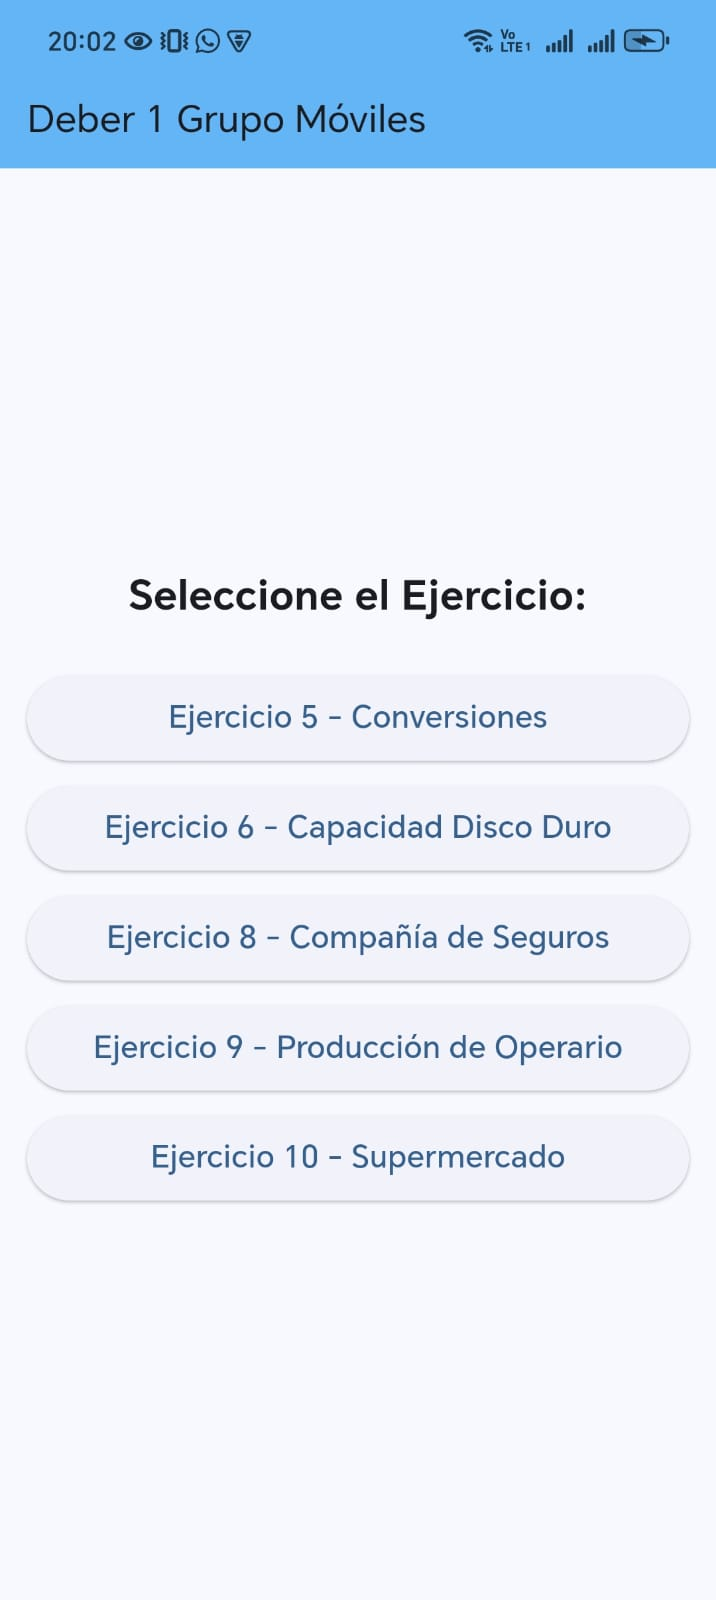
\includegraphics[width=\linewidth]{img/menu.jpeg}
  \captionof{anexofloat}{Menú principal de la aplicación}
\end{minipage}
\hfill
\begin{minipage}[t]{0.45\textwidth}
  \centering
  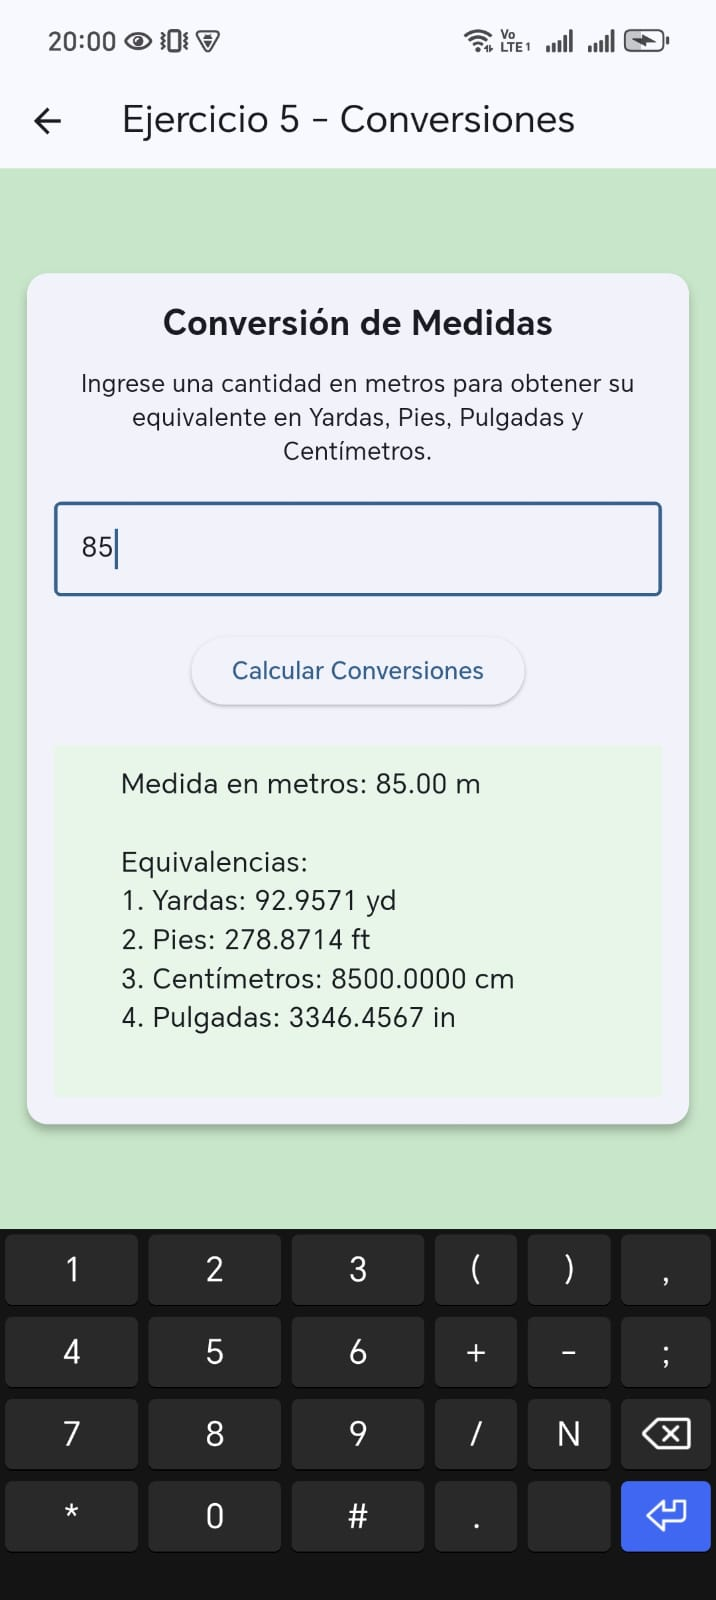
\includegraphics[width=\linewidth]{img/ejercicio5.jpeg}
  \captionof{anexofloat}{Ejercicio 5 -- Conversión de Medidas}
\end{minipage}

\vspace{1.2cm}

% --- Fila 2 ---
\noindent
\begin{minipage}[t]{0.45\textwidth}
  \centering
  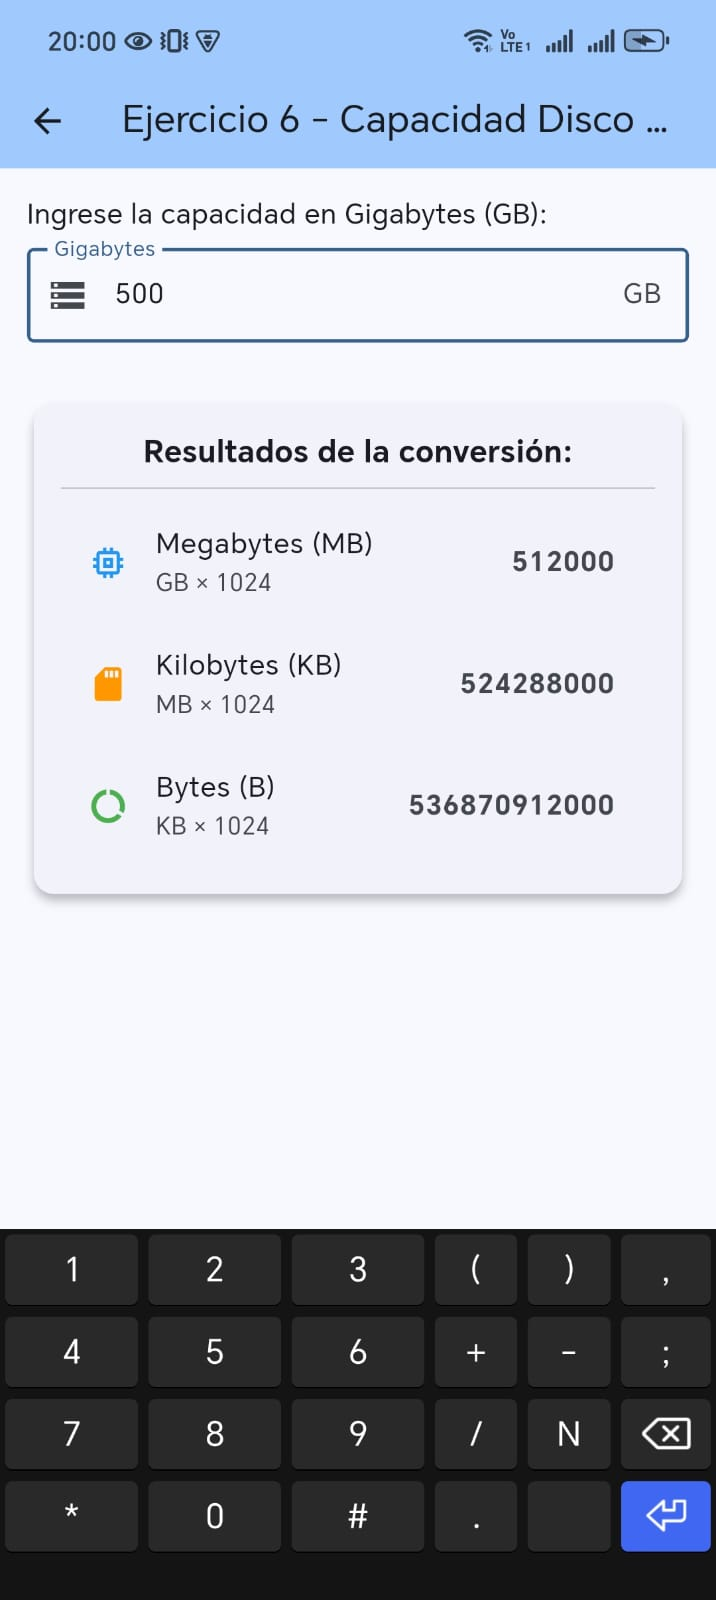
\includegraphics[width=\linewidth]{img/ejercicio6.jpeg}
  \captionof{anexofloat}{Ejercicio 6 -- Capacidad de Disco Duro}
\end{minipage}
\hfill
\begin{minipage}[t]{0.45\textwidth}
  \centering
  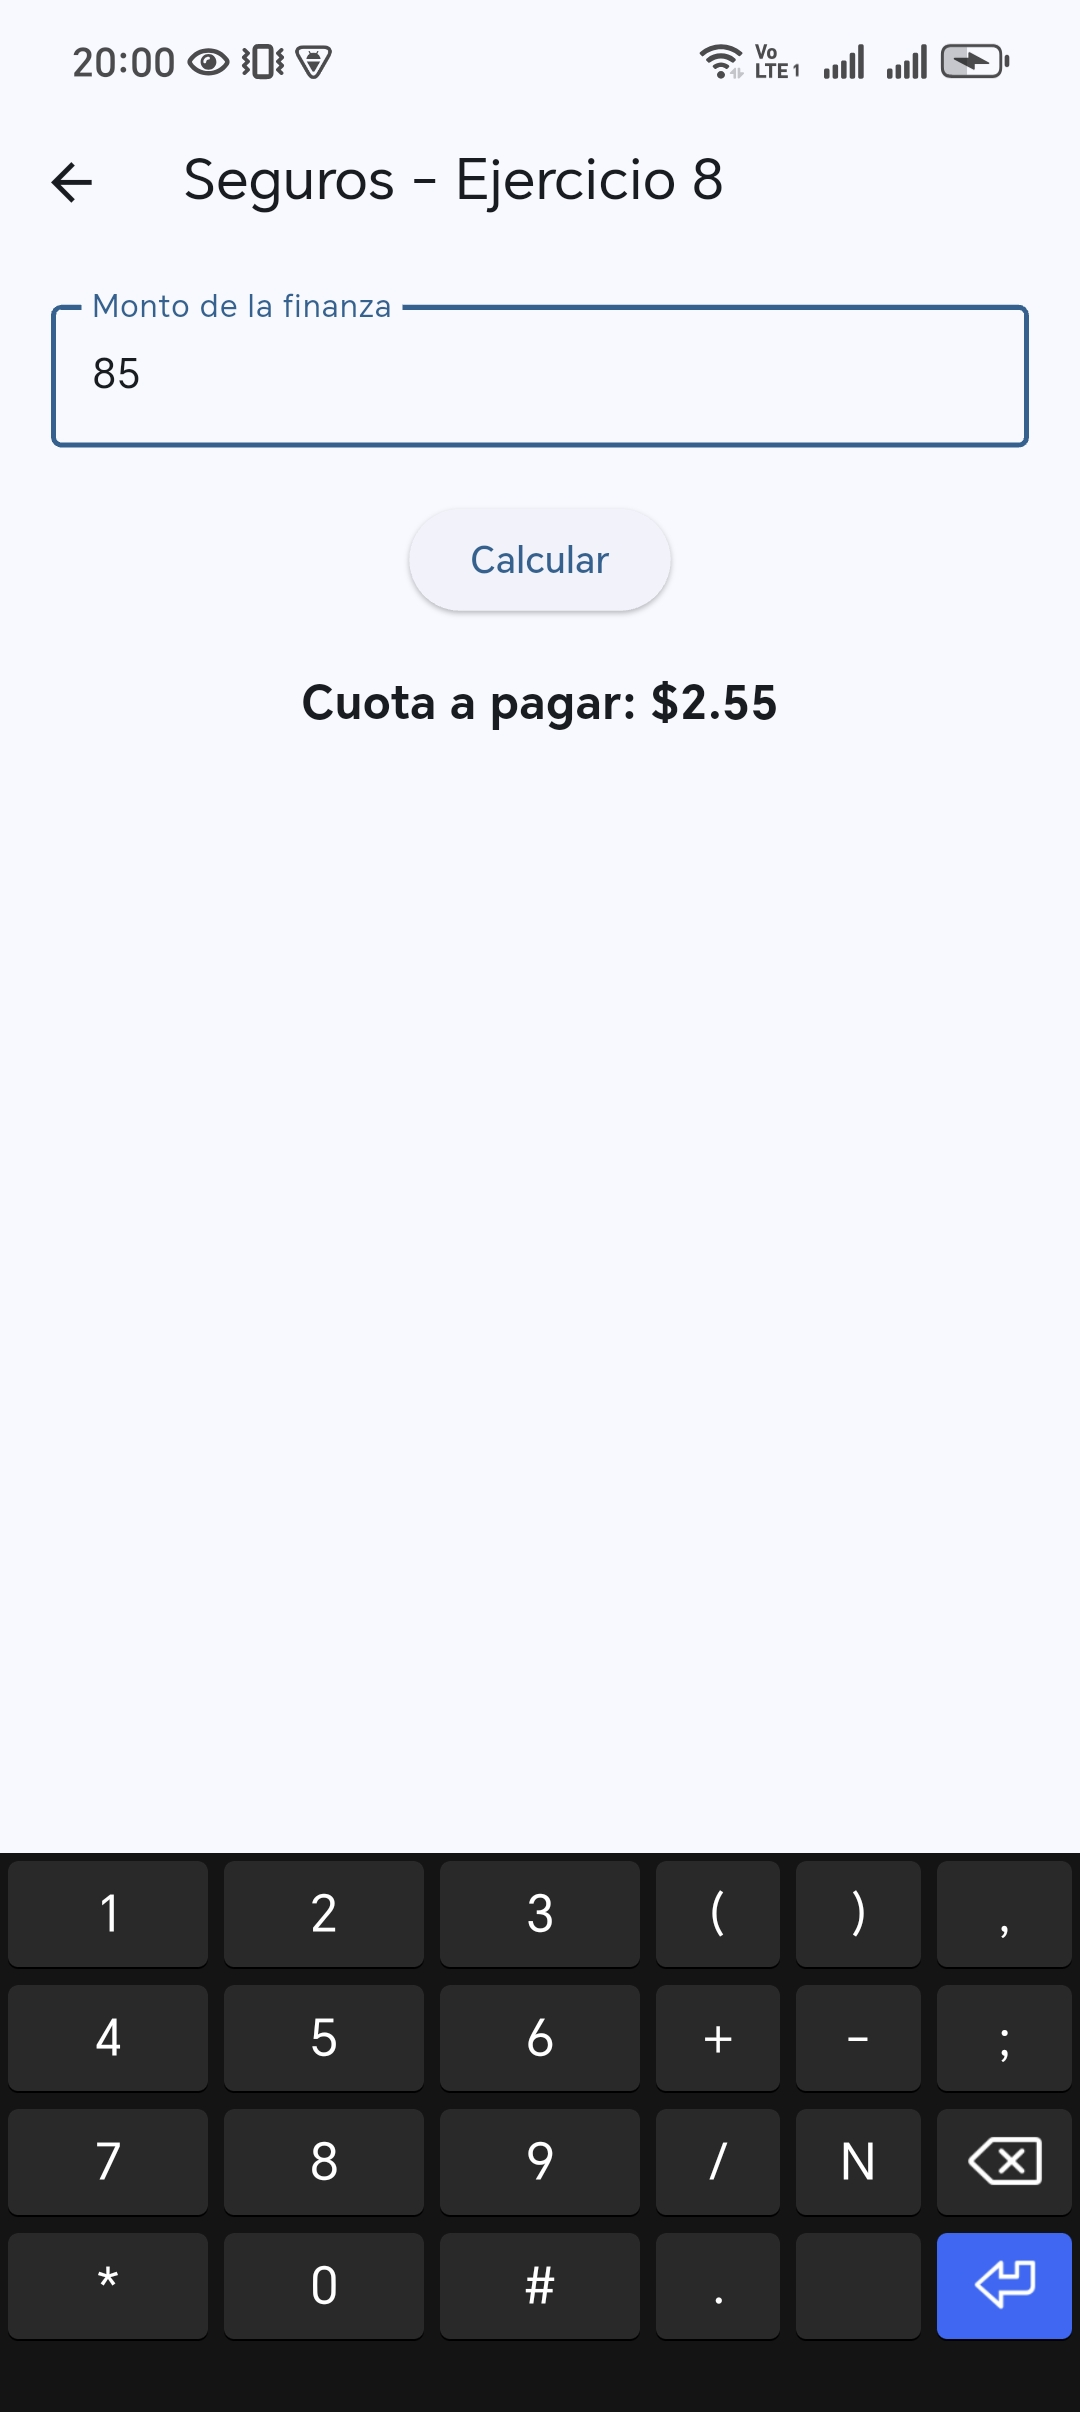
\includegraphics[width=\linewidth]{img/ejercicio8.jpeg}
  \captionof{anexofloat}{Ejercicio 8 -- Compañía de Seguros}
\end{minipage}

\vspace{1.2cm}

% --- Fila 3 ---
\noindent
\begin{minipage}[t]{0.45\textwidth}
  \centering
  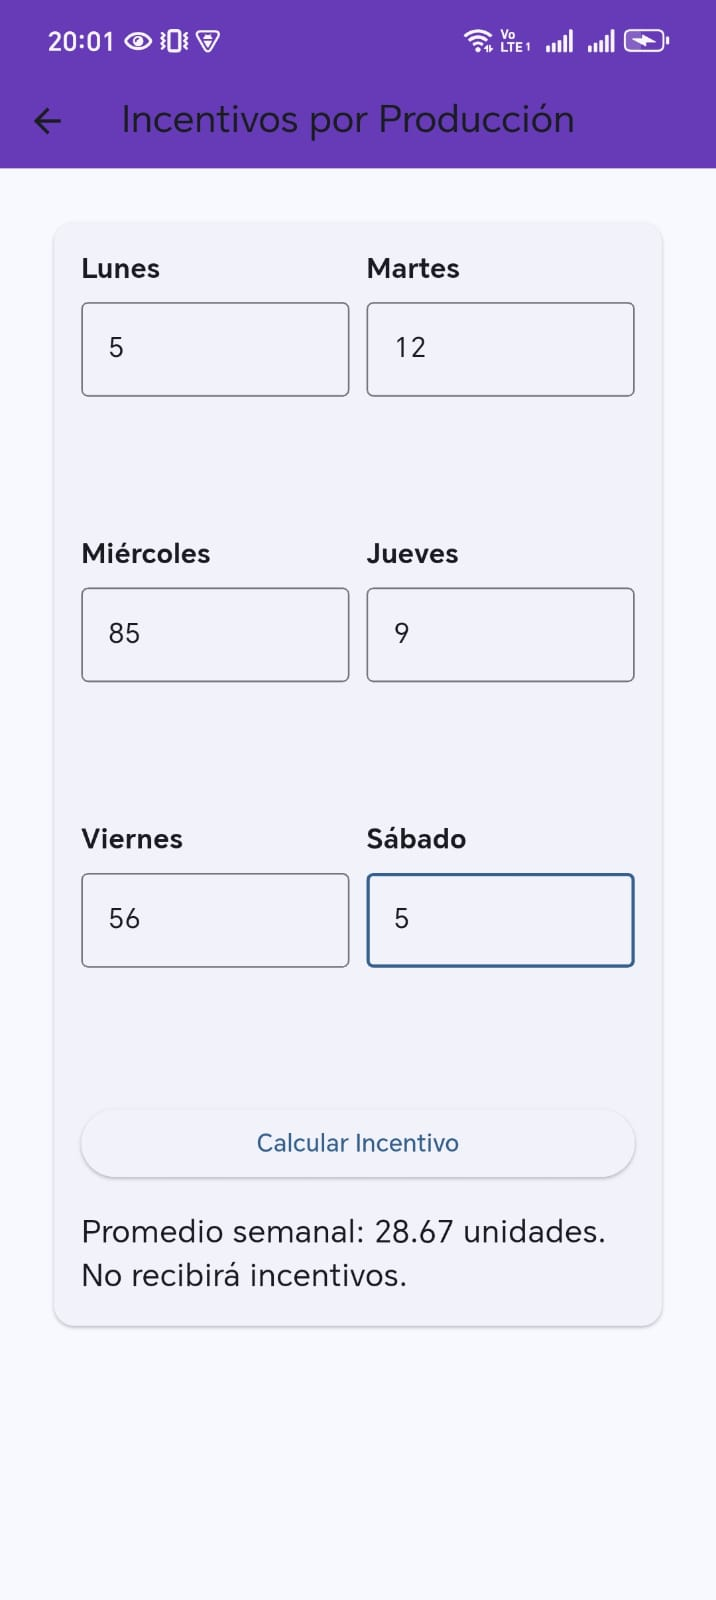
\includegraphics[width=\linewidth]{img/ejercicio9.jpeg}
  \captionof{anexofloat}{Ejercicio 9 -- Producción de Operario}
\end{minipage}
\hfill
\begin{minipage}[t]{0.45\textwidth}
  \centering
  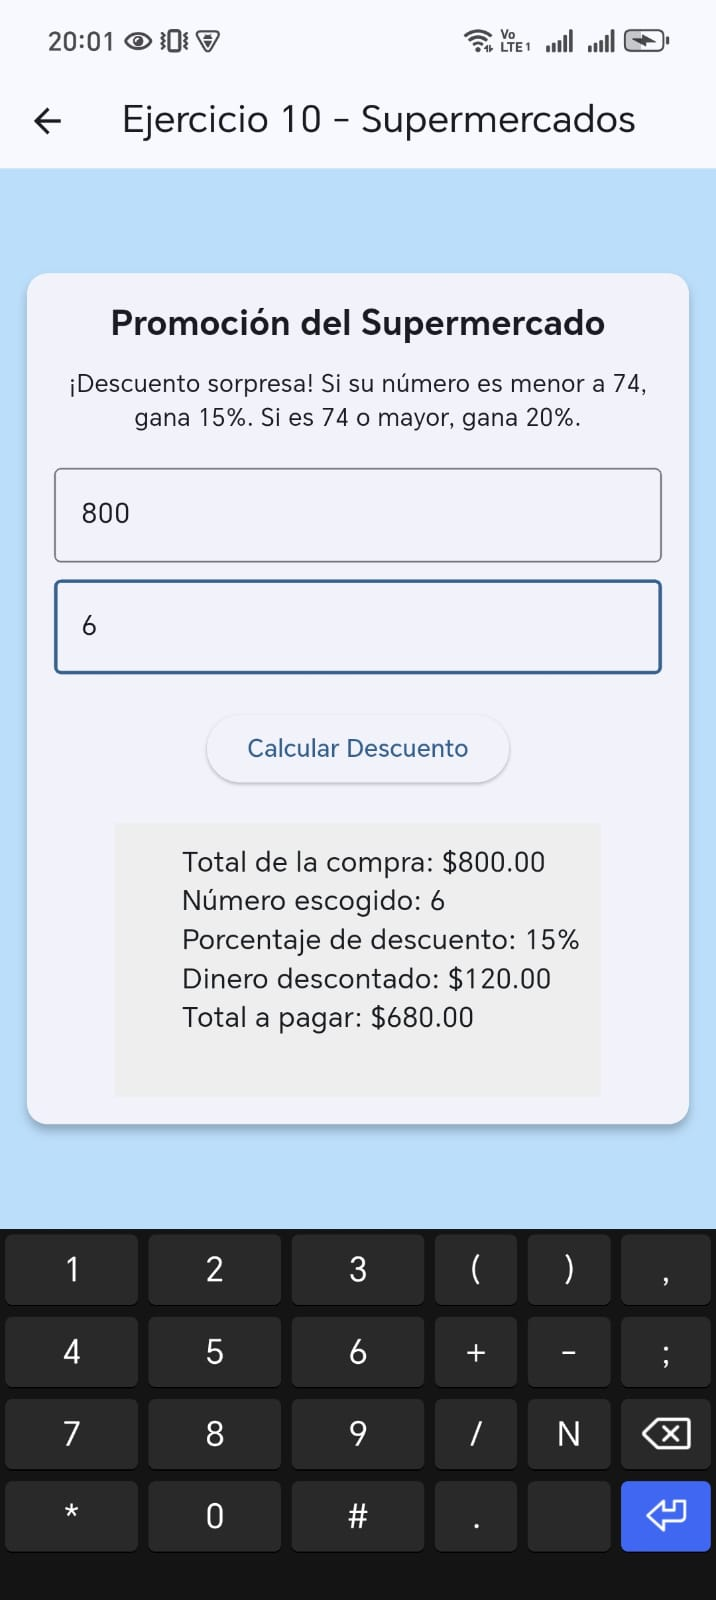
\includegraphics[width=\linewidth]{img/ejercicio10.jpeg}
  \captionof{anexofloat}{Ejercicio 10 -- Supermercado}
\end{minipage}

\end{document}
